% !TEX TS-program = pdflatex
% !TEX encoding = UTF-8 Unicode

% This is a simple template for a LaTeX document using the "article" class.
% See "book", "report", "letter" for other types of document.

\documentclass[11pt]{article} % use larger type; default would be 10pt


\usepackage{ulem}
\newcommand\NoIndent[1]{%
  \par\vbox{\parbox[t]{\linewidth}{#1}}%
}


\usepackage[utf8]{inputenc} % set input encoding (not needed with XeLaTeX)

%%% Examples of Article customizations
% These packages are optional, depending whether you want the features they provide.
% See the LaTeX Companion or other references for full information.

%%% PAGE DIMENSIONS
\usepackage{geometry} % to change the page dimensions
\geometry{a4paper} % or letterpaper (US) or a5paper or....
% \geometry{margin=2in} % for example, change the margins to 2 inches all round
% \geometry{landscape} % set up the page for landscape
%   read geometry.pdf for detailed page layout information

\usepackage{graphicx} % support the \includegraphics command and options

% \usepackage[parfill]{parskip} % Activate to begin paragraphs with an empty line rather than an indent

%%% PACKAGES
\usepackage{booktabs} % for much better looking tables
\usepackage{array} % for better arrays (eg matrices) in maths
\usepackage{paralist} % very flexible & customisable lists (eg. enumerate/itemize, etc.)
\usepackage{verbatim} % adds environment for commenting out blocks of text & for better verbatim
\usepackage{subfig} % make it possible to include more than one captioned figure/table in a single float
% These packages are all incorporated in the memoir class to one degree or another...

%%% HEADERS & FOOTERS
\usepackage{fancyhdr} % This should be set AFTER setting up the page geometry
\pagestyle{fancy} % options: empty , plain , fancy
\renewcommand{\headrulewidth}{0pt} % customise the layout...
\lhead{}\chead{}\rhead{}
\lfoot{}\cfoot{\thepage}\rfoot{}

%%% SECTION TITLE APPEARANCE
\usepackage{sectsty}
\allsectionsfont{\sffamily\mdseries\upshape} % (See the fntguide.pdf for font help)
% (This matches ConTeXt defaults)

%%% ToC (table of contents) APPEARANCE
\usepackage[nottoc,notlof,notlot]{tocbibind} % Put the bibliography in the ToC
\usepackage[titles,subfigure]{tocloft} % Alter the style of the Table of Contents
\renewcommand{\cftsecfont}{\rmfamily\mdseries\upshape}
\renewcommand{\cftsecpagefont}{\rmfamily\mdseries\upshape} % No bold!

%%% END Article customizations


\usepackage{verbatim}
\usepackage{amsmath}


\title{Work Log for November}
\author{Logan Brown}
%\date{} % Activate to display a given date or no date (if empty),
         % otherwise the current date is printed 

\begin{document}
\maketitle
\tableofcontents

\newpage


\section{Goals for the Month}
As of October 31st
\begin{enumerate}
\item Use Preston's Simulated Yeast, compare to REU yeast

look for estimated $\approx$ 4*true
\item Parallelize the Code

mclapply, getOption(``mc.cores")?
\item Wei Chen's Yeast / Real Yeast Genome
\item Generate my own simulated yeast, using a reverse engineered cubfits
\end{enumerate}

%Paste output from writeGoals
\section{Progress/Notes}

\subsection{Use Preston's Simulated Yeast, compare to REU yeast}

Here are the results from Preston's simulated yeast...

Notice that the $\Delta\omega$ values are not off by that $\approx4$ factor. We got a pretty good correlation on the log$\mu$ values, but the $\phi$ is pretty lousy, and the $\omega$ values leave something to be desired.

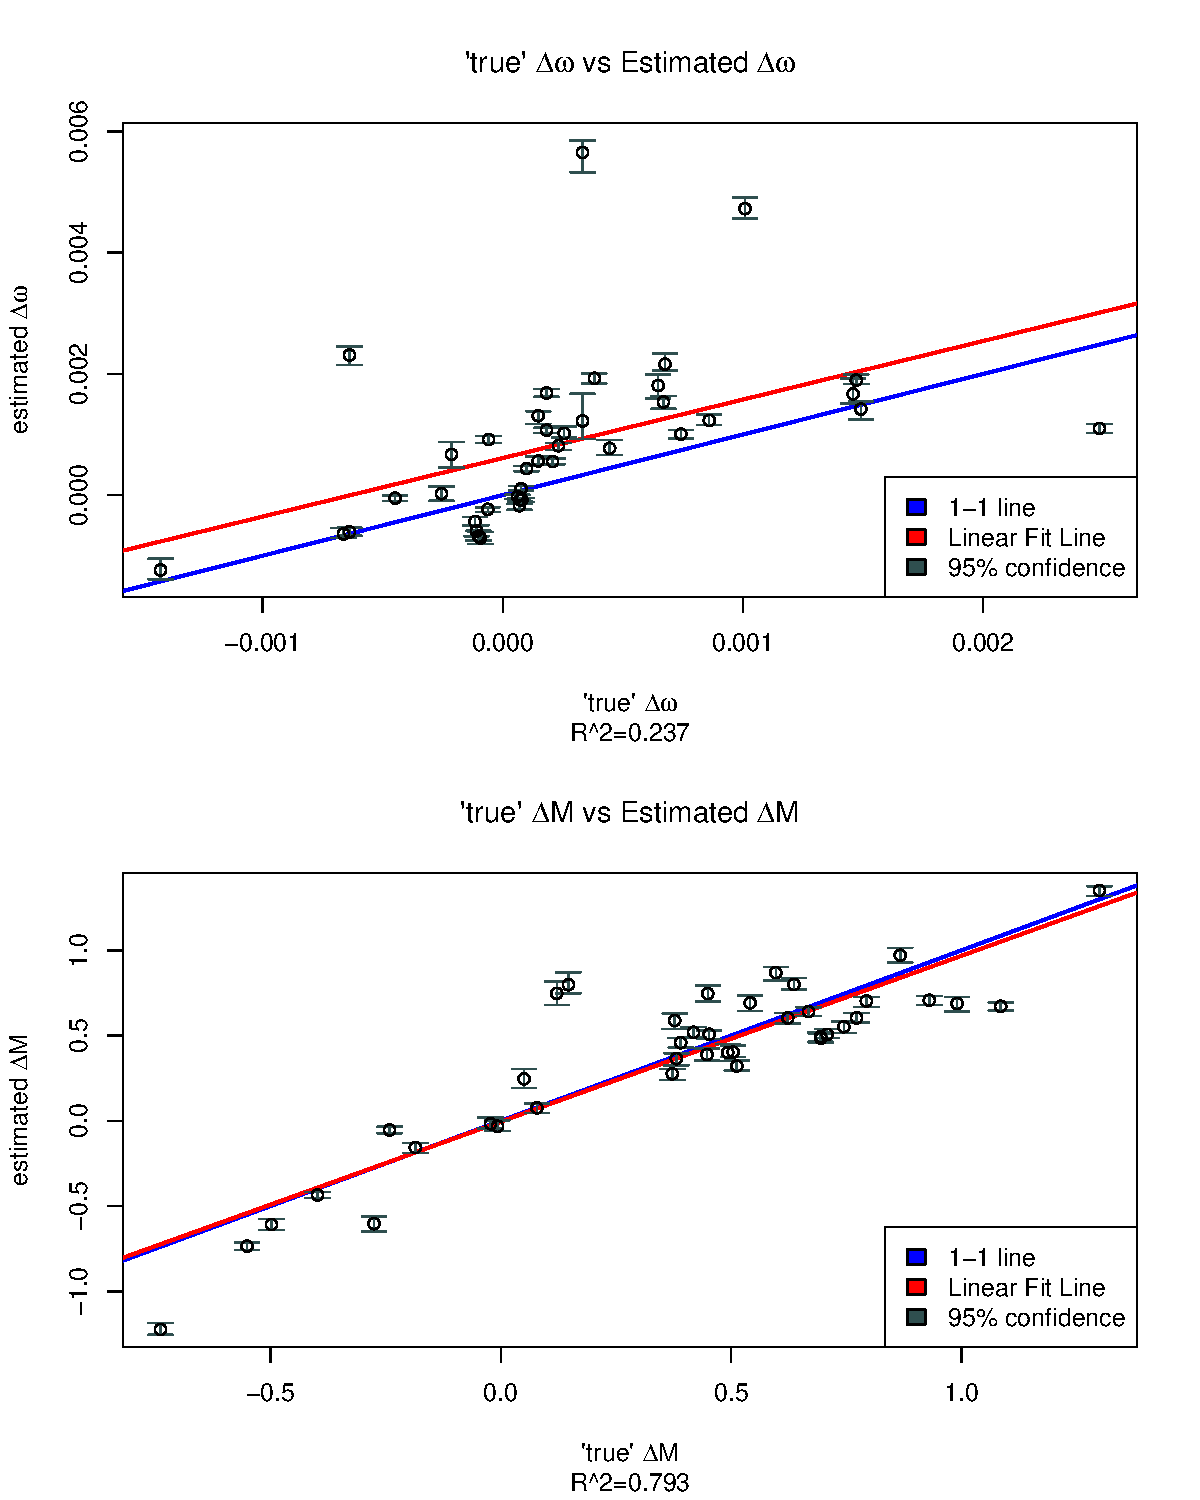
\includepdf[pages={1}]{data/1105_codonParameters_8core.pdf}
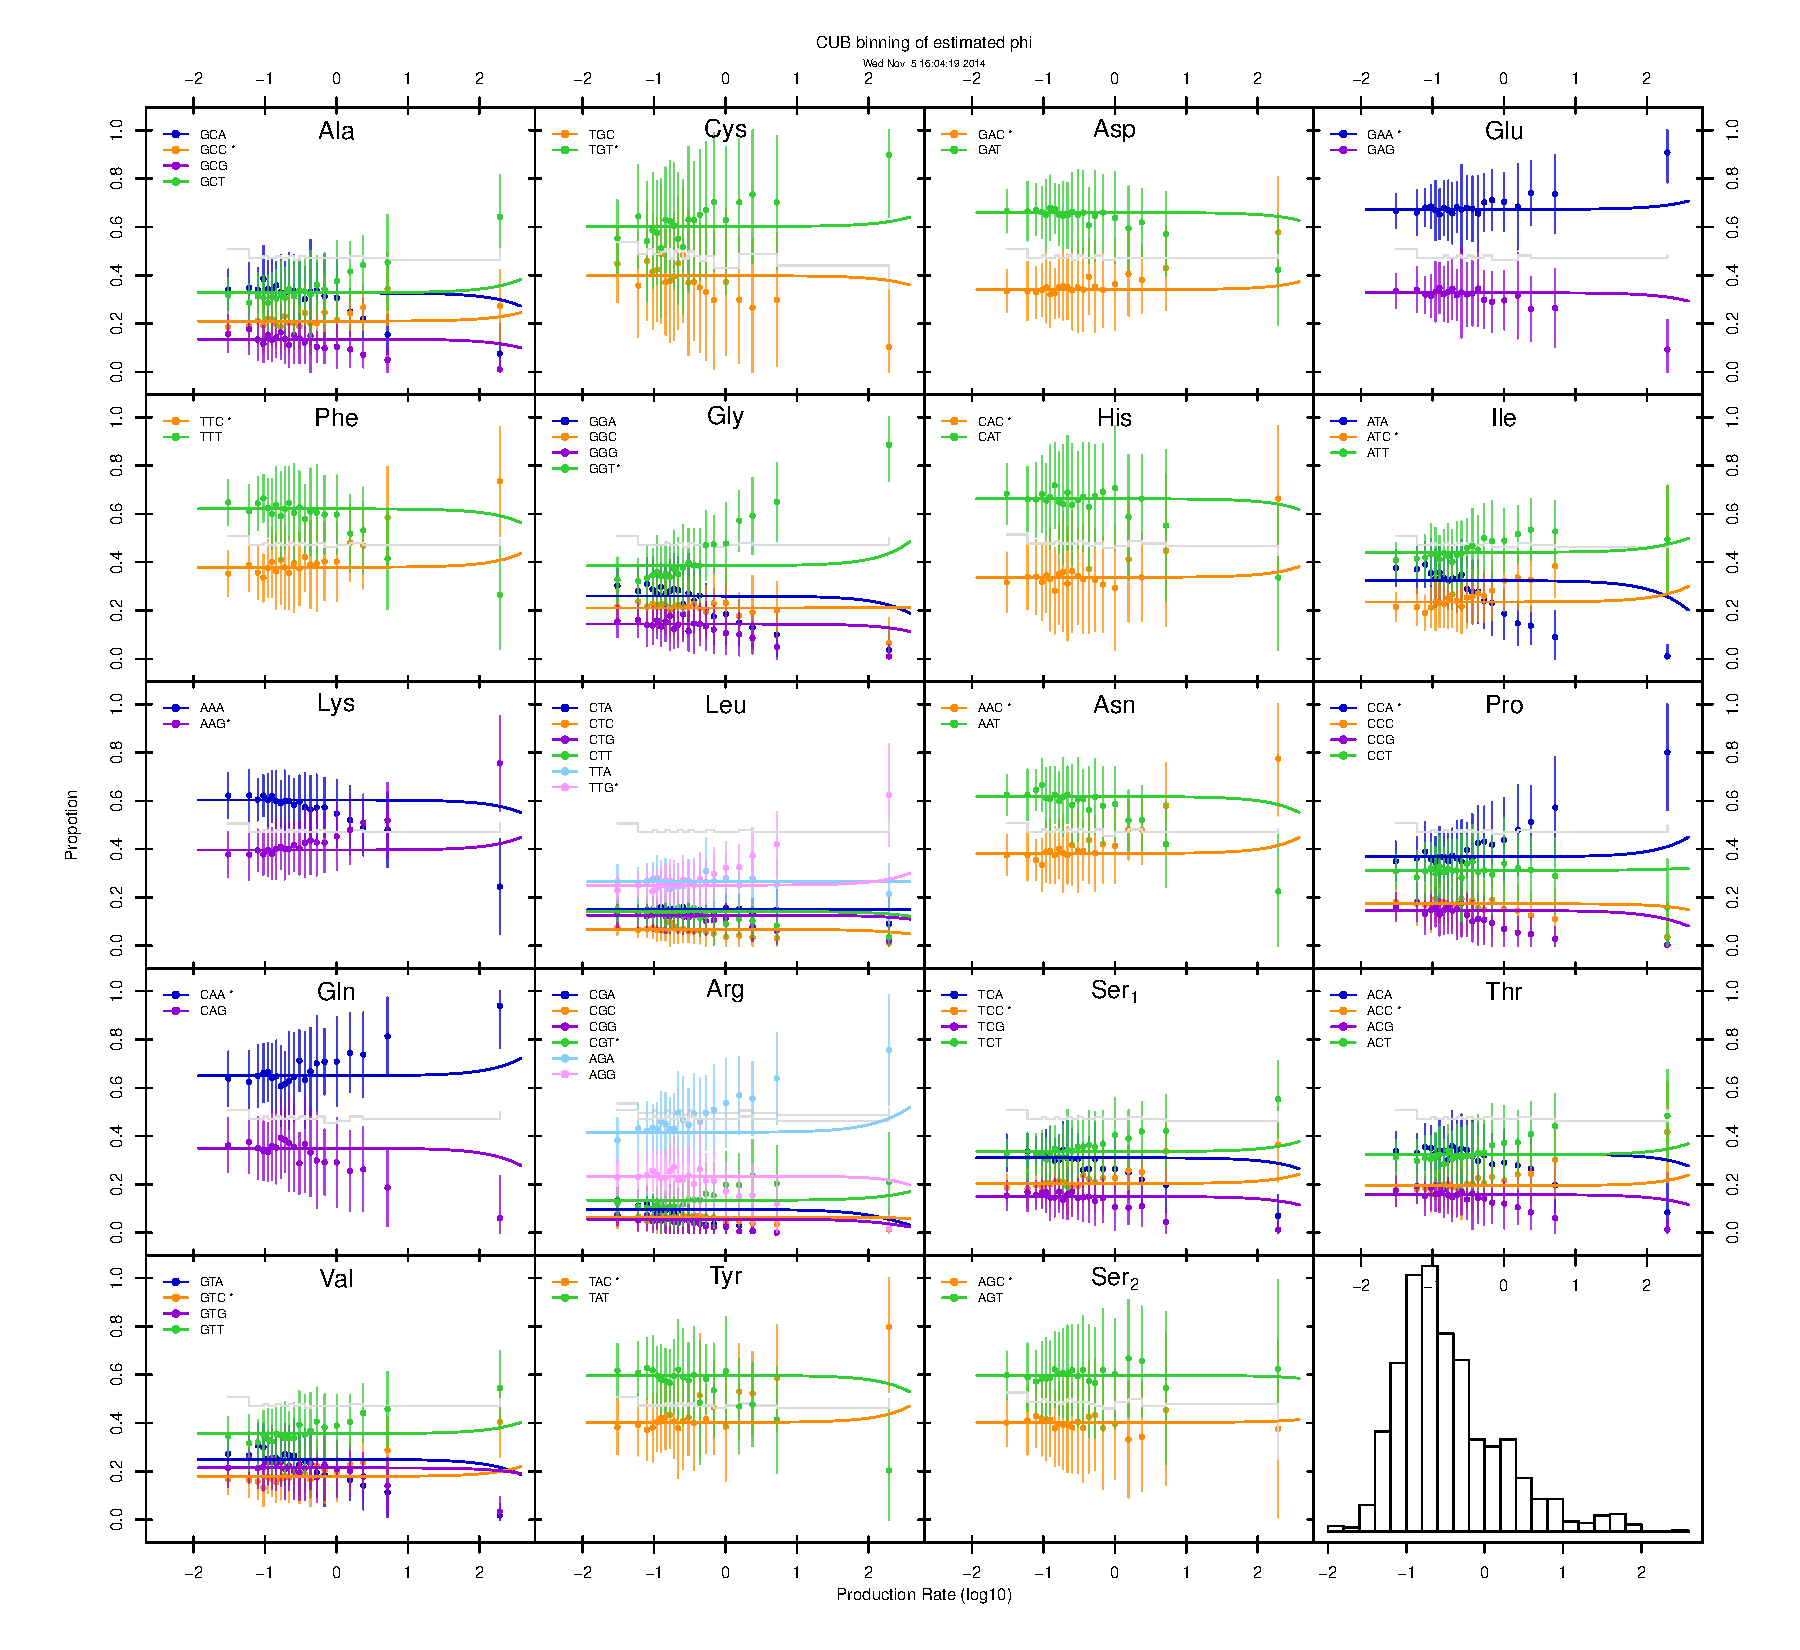
\includepdf[pages={1}]{data/1105_CUB_est_bin_8core.pdf}
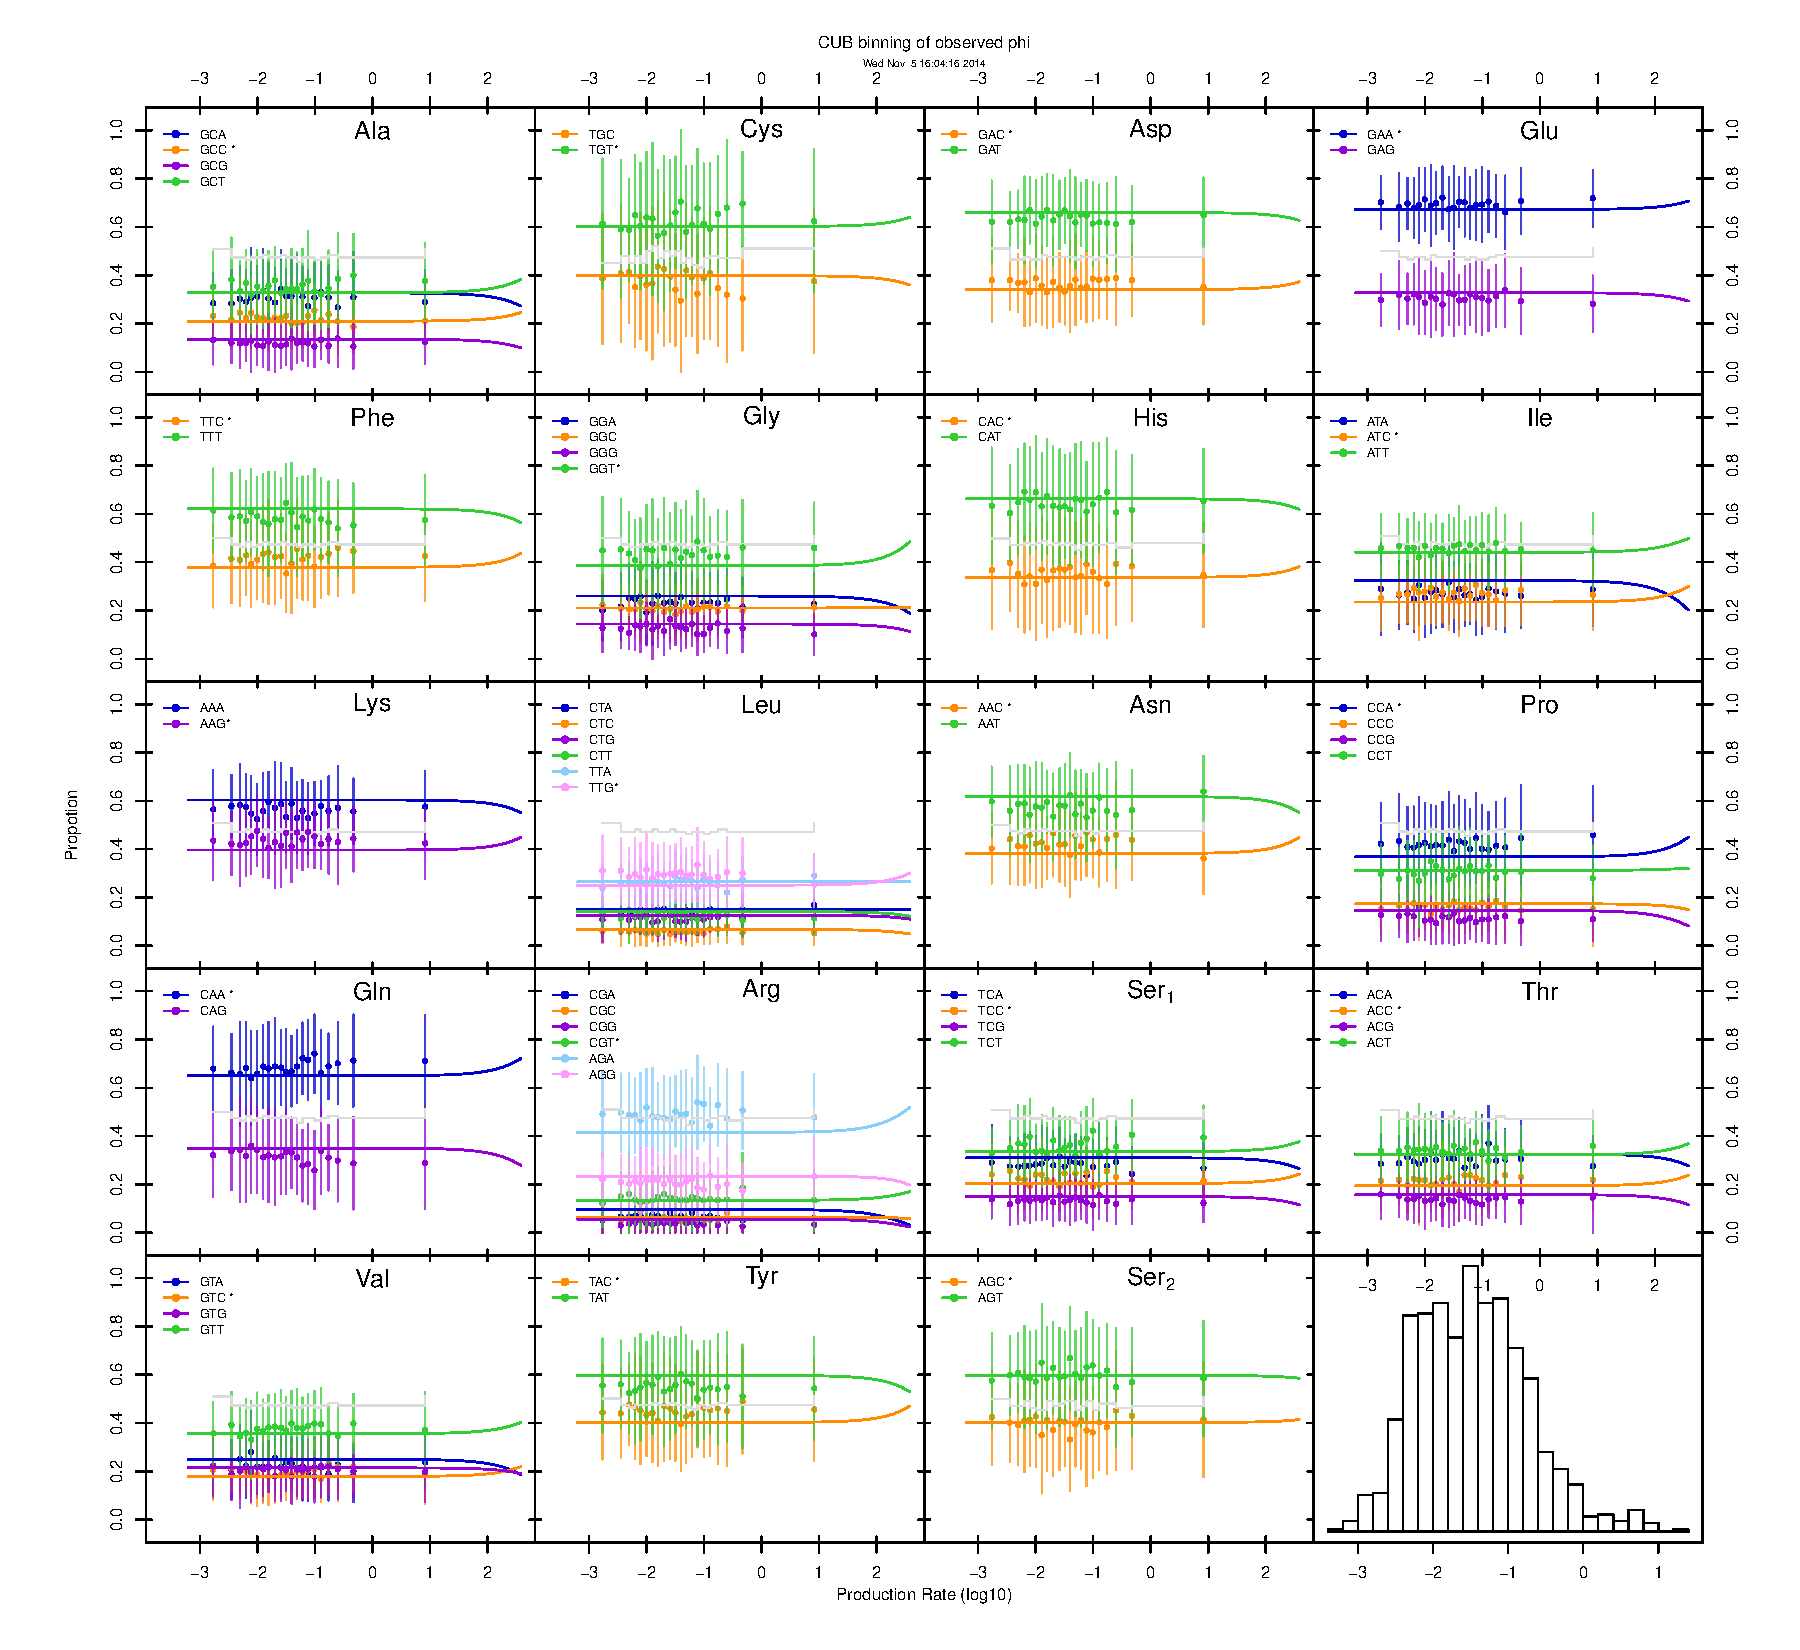
\includepdf[pages={1}]{data/1105_CUB_obs_bin_8core.pdf}
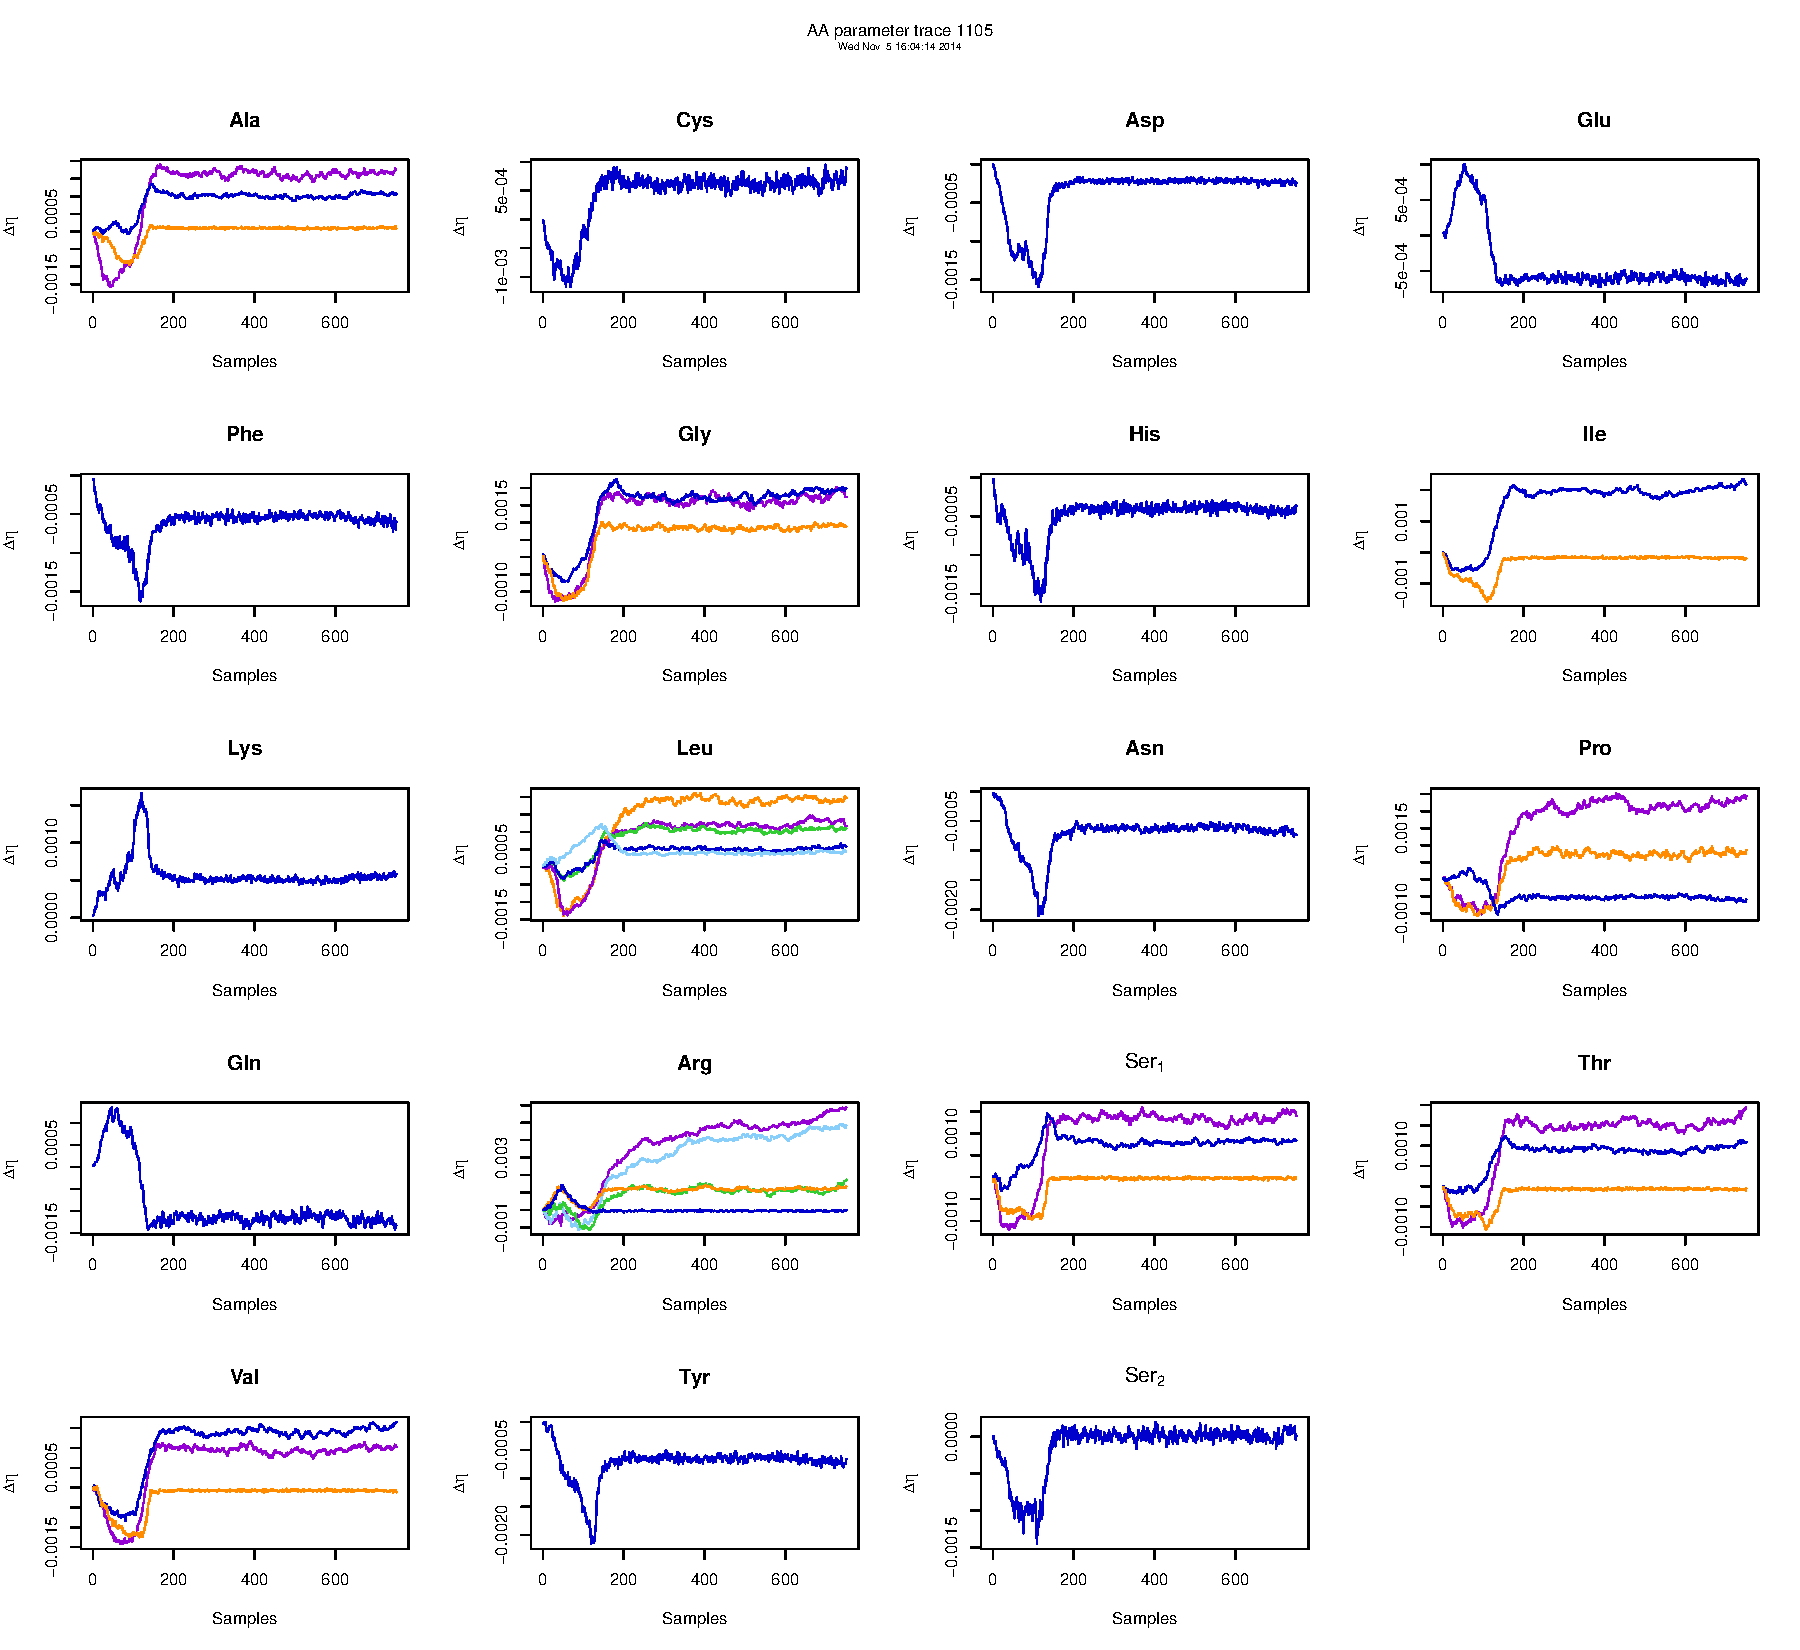
\includepdf[pages={1}]{data/1105_deltaeta_8core.pdf}
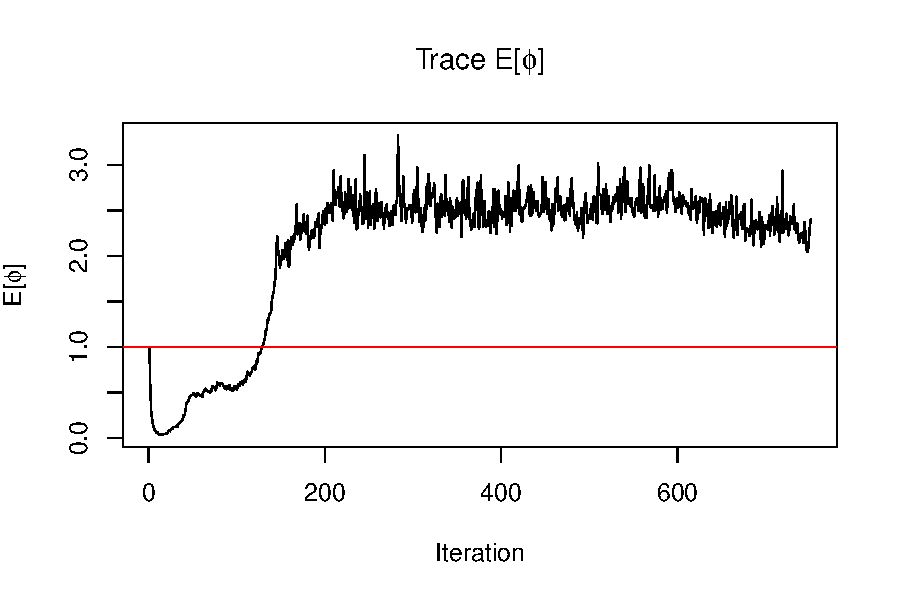
\includepdf[pages={1}]{data/1105_expPhi_trace_8core.pdf}
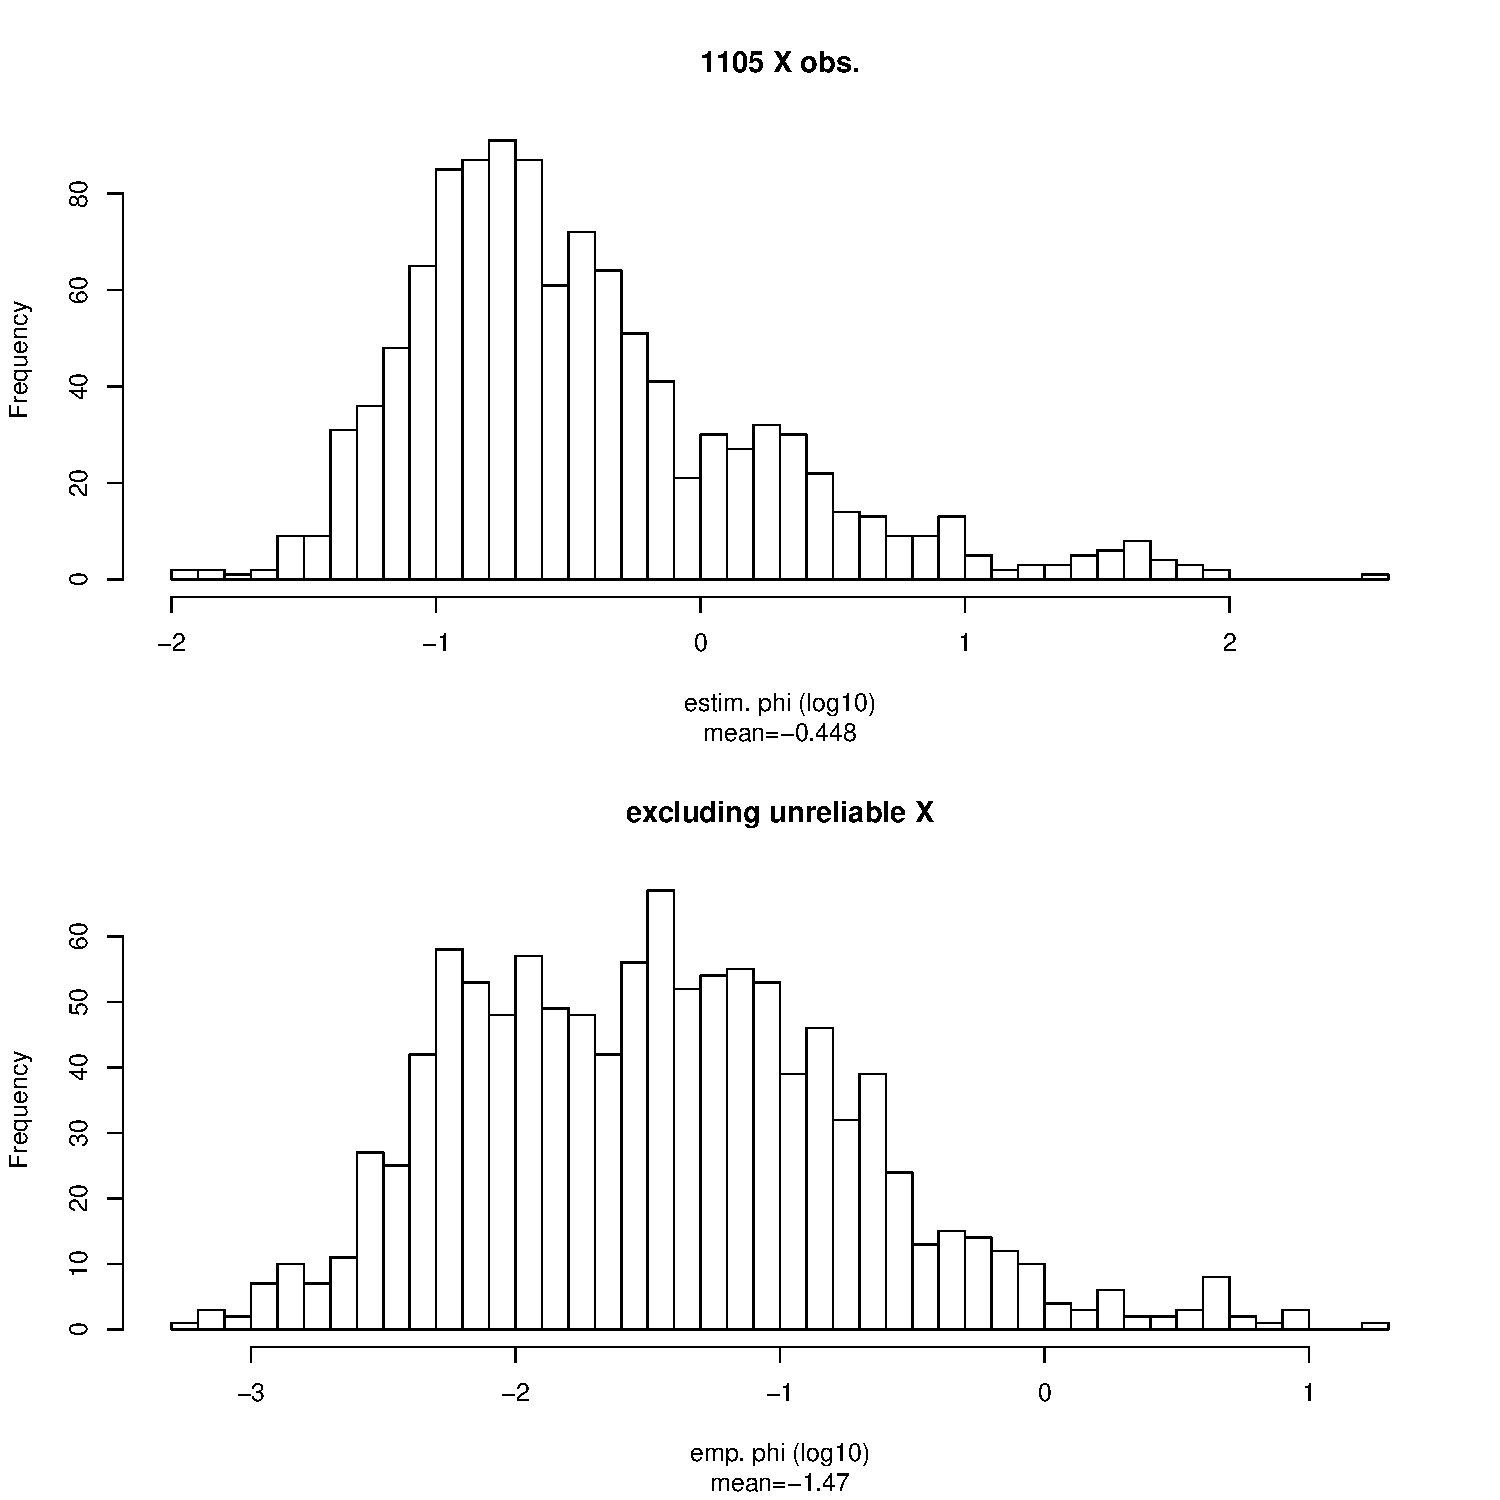
\includepdf[pages={1}]{data/1105_histogram_8core.pdf}
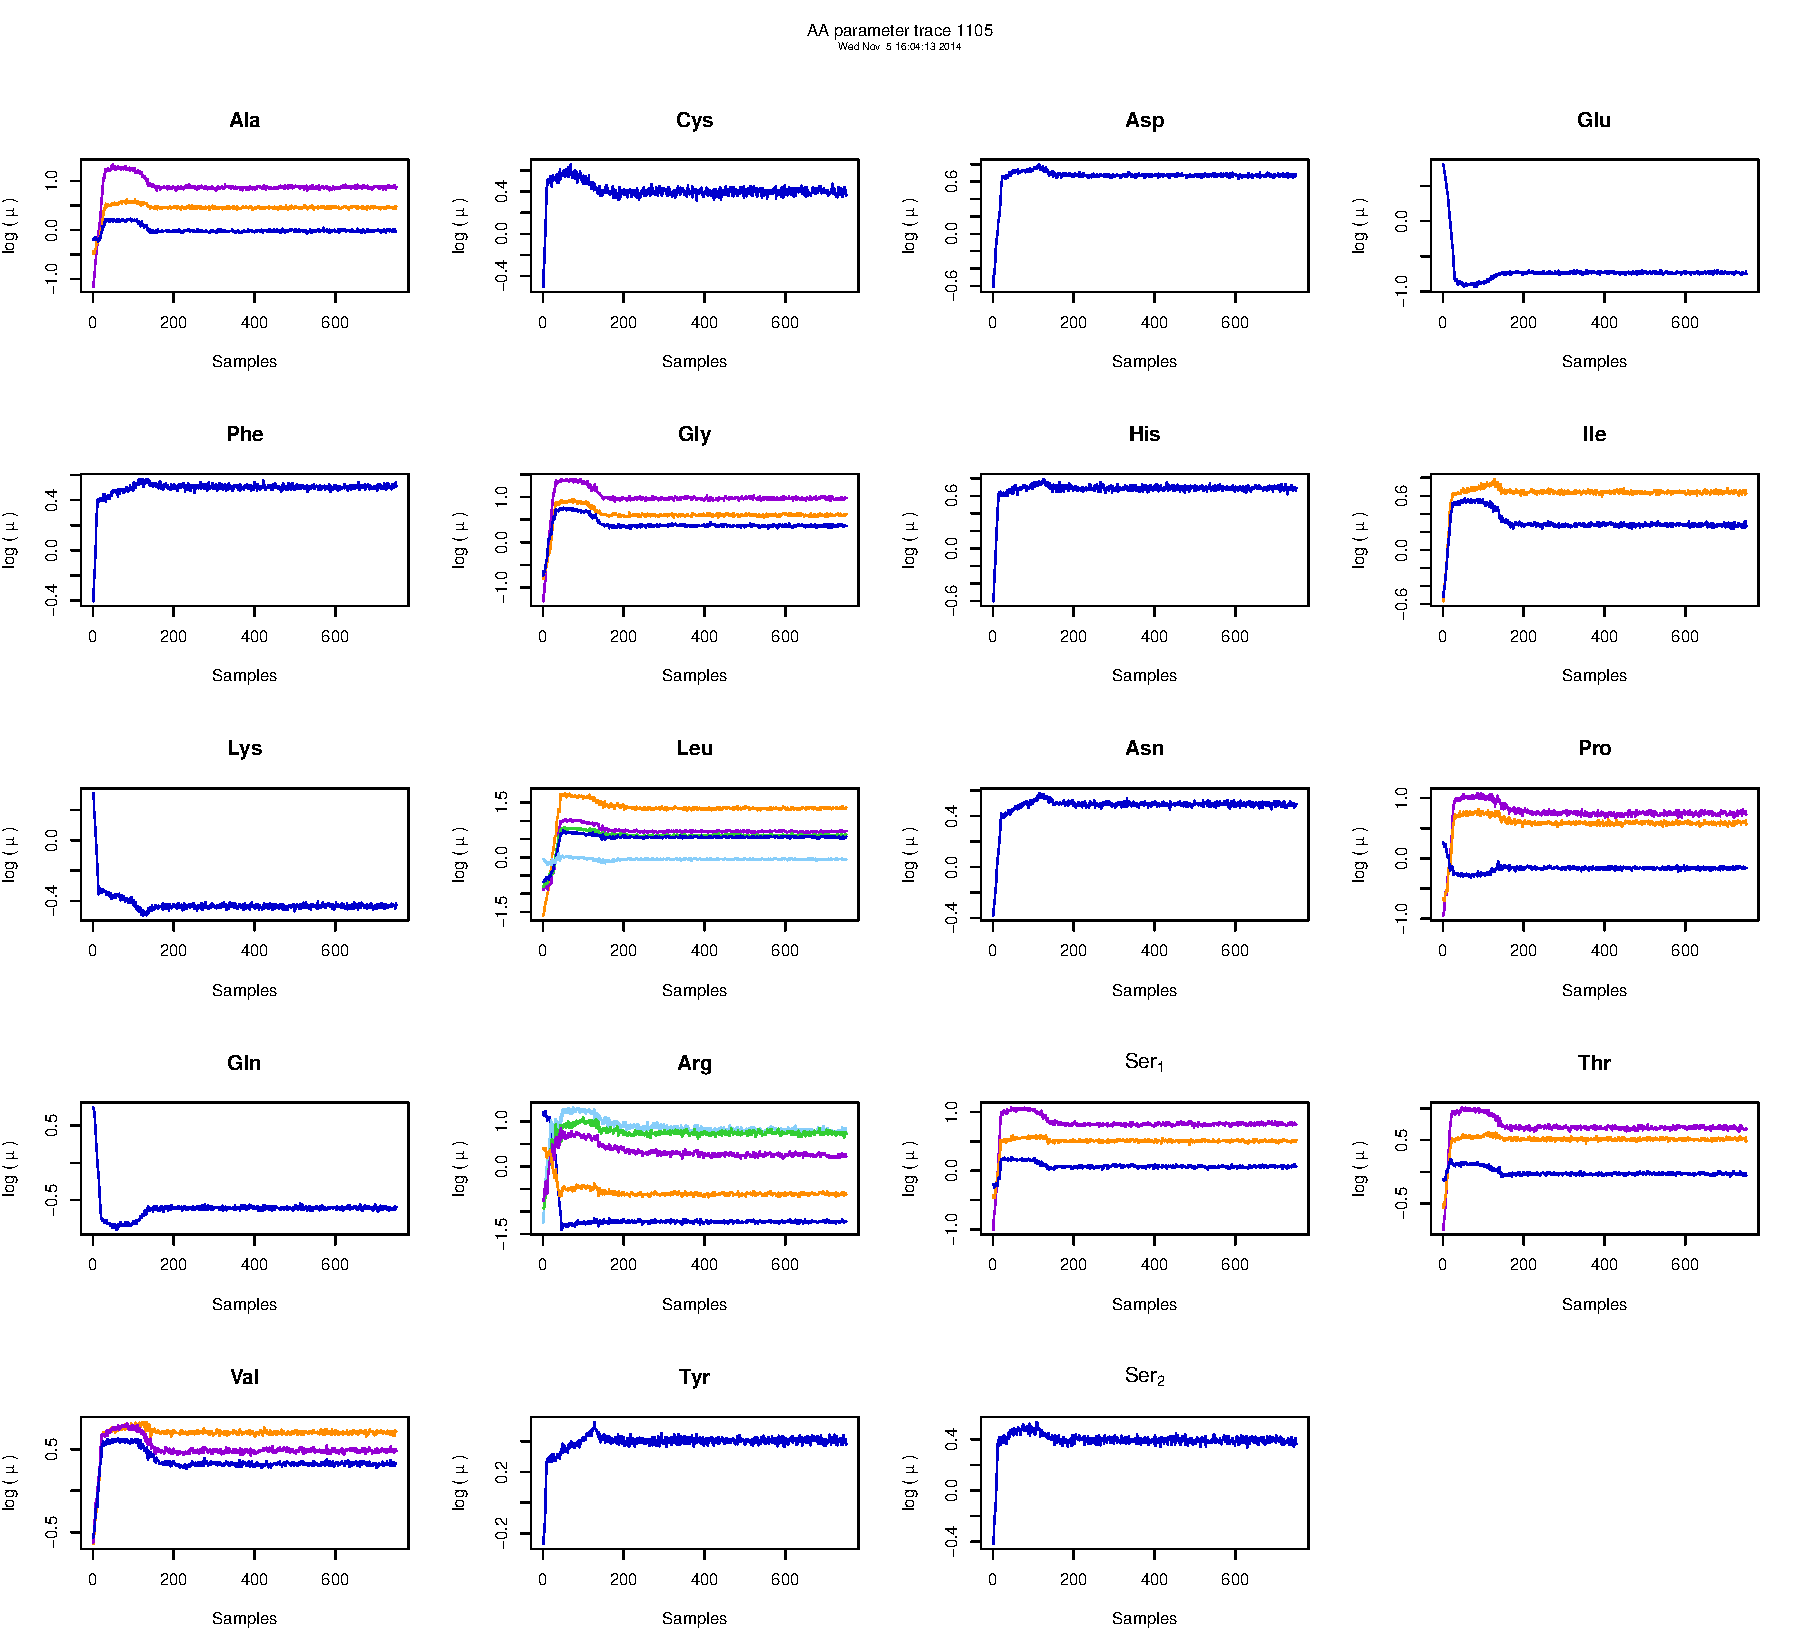
\includepdf[pages={1}]{data/1105_logmu_8core.pdf}
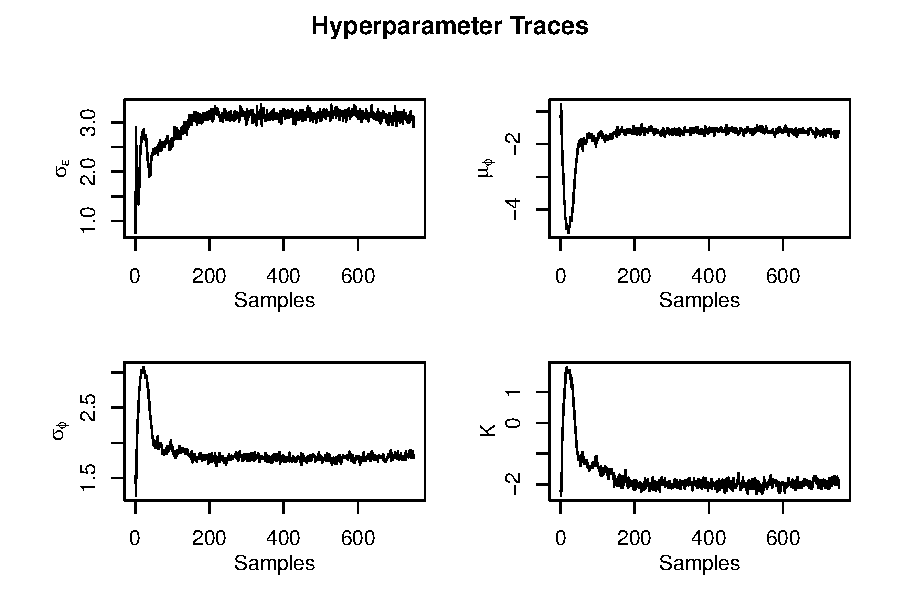
\includepdf[pages={1}]{data/1105_pMat_trace_8core.pdf}
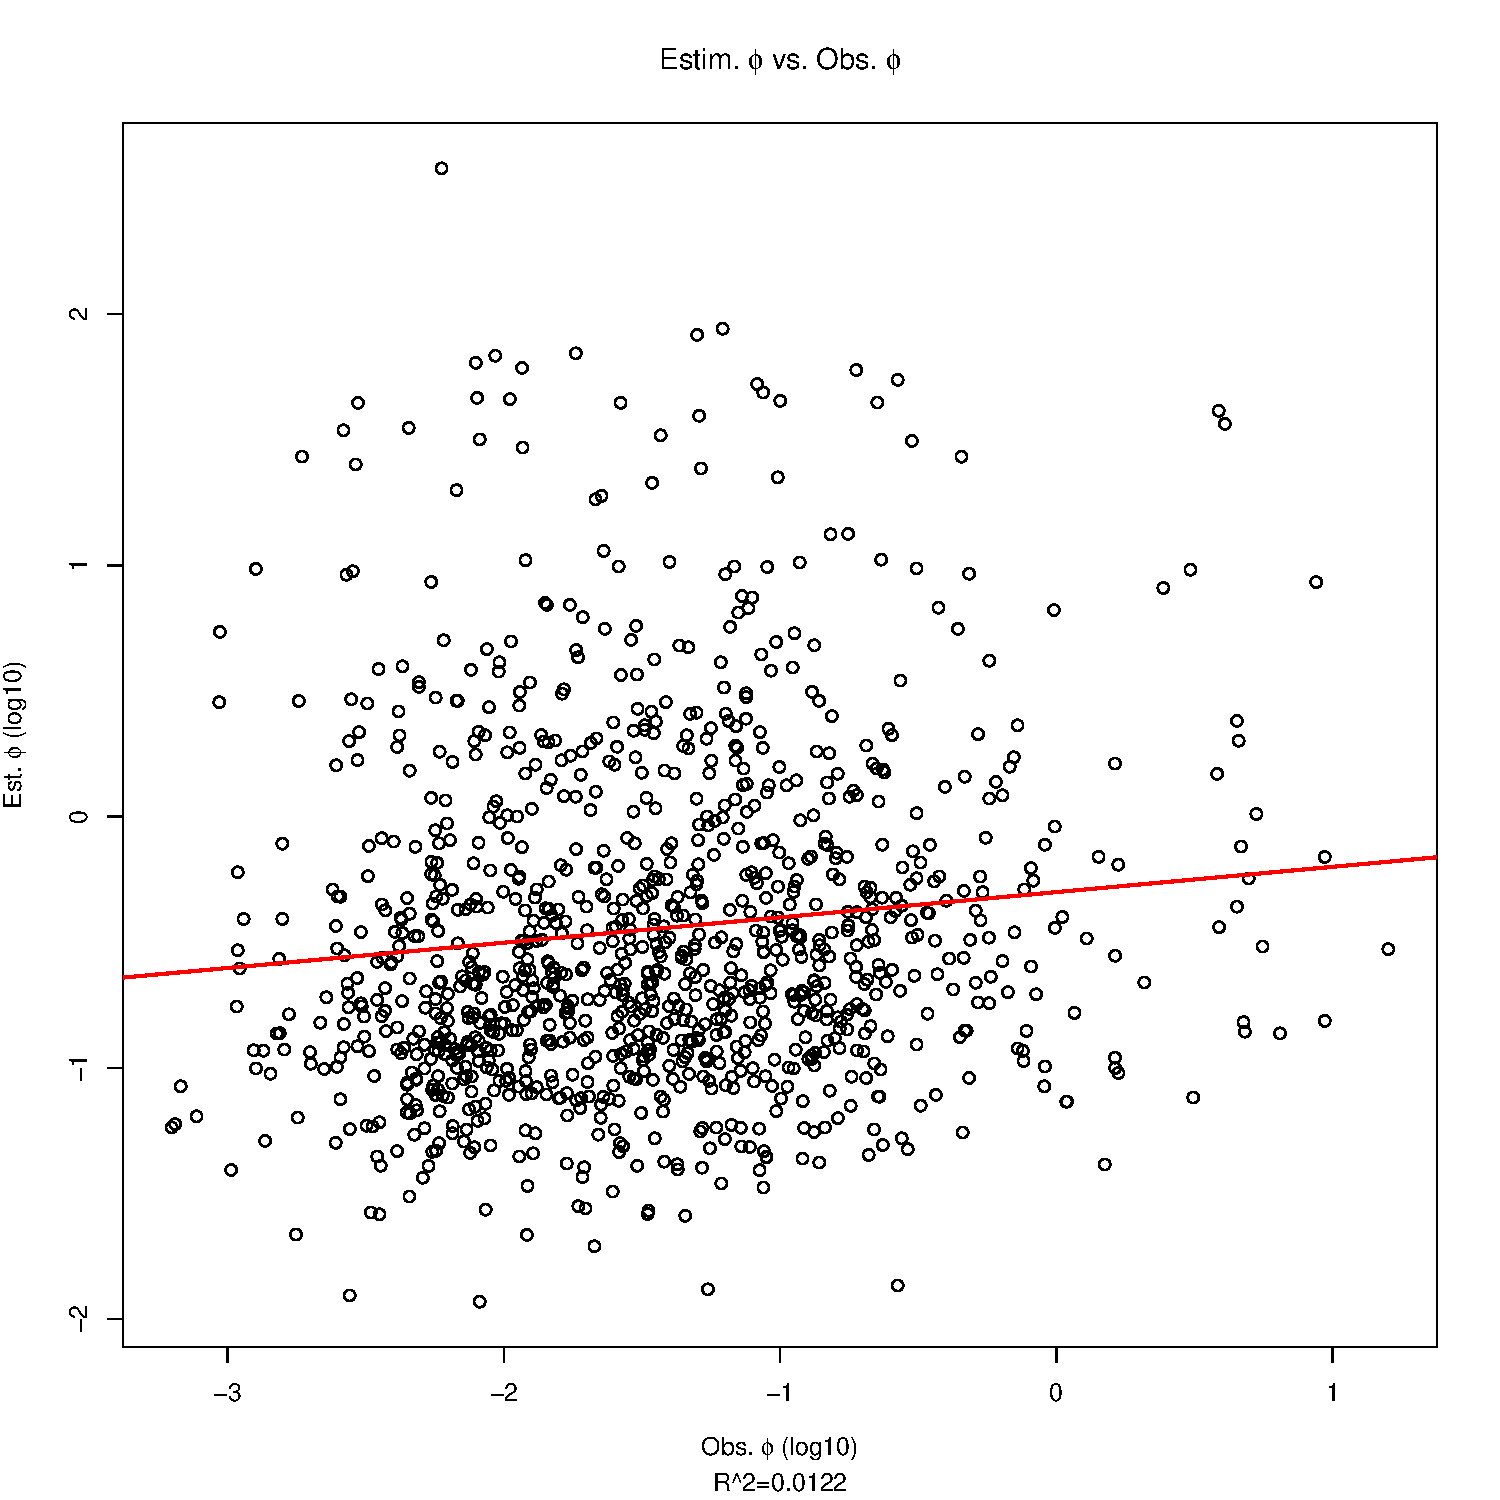
\includepdf[pages={1}]{data/1105_vs_obs_phi_8core.pdf}

Note how different the $\Delta\omega$ values are between Preston's yeast genome and the REU students' yeast genome.

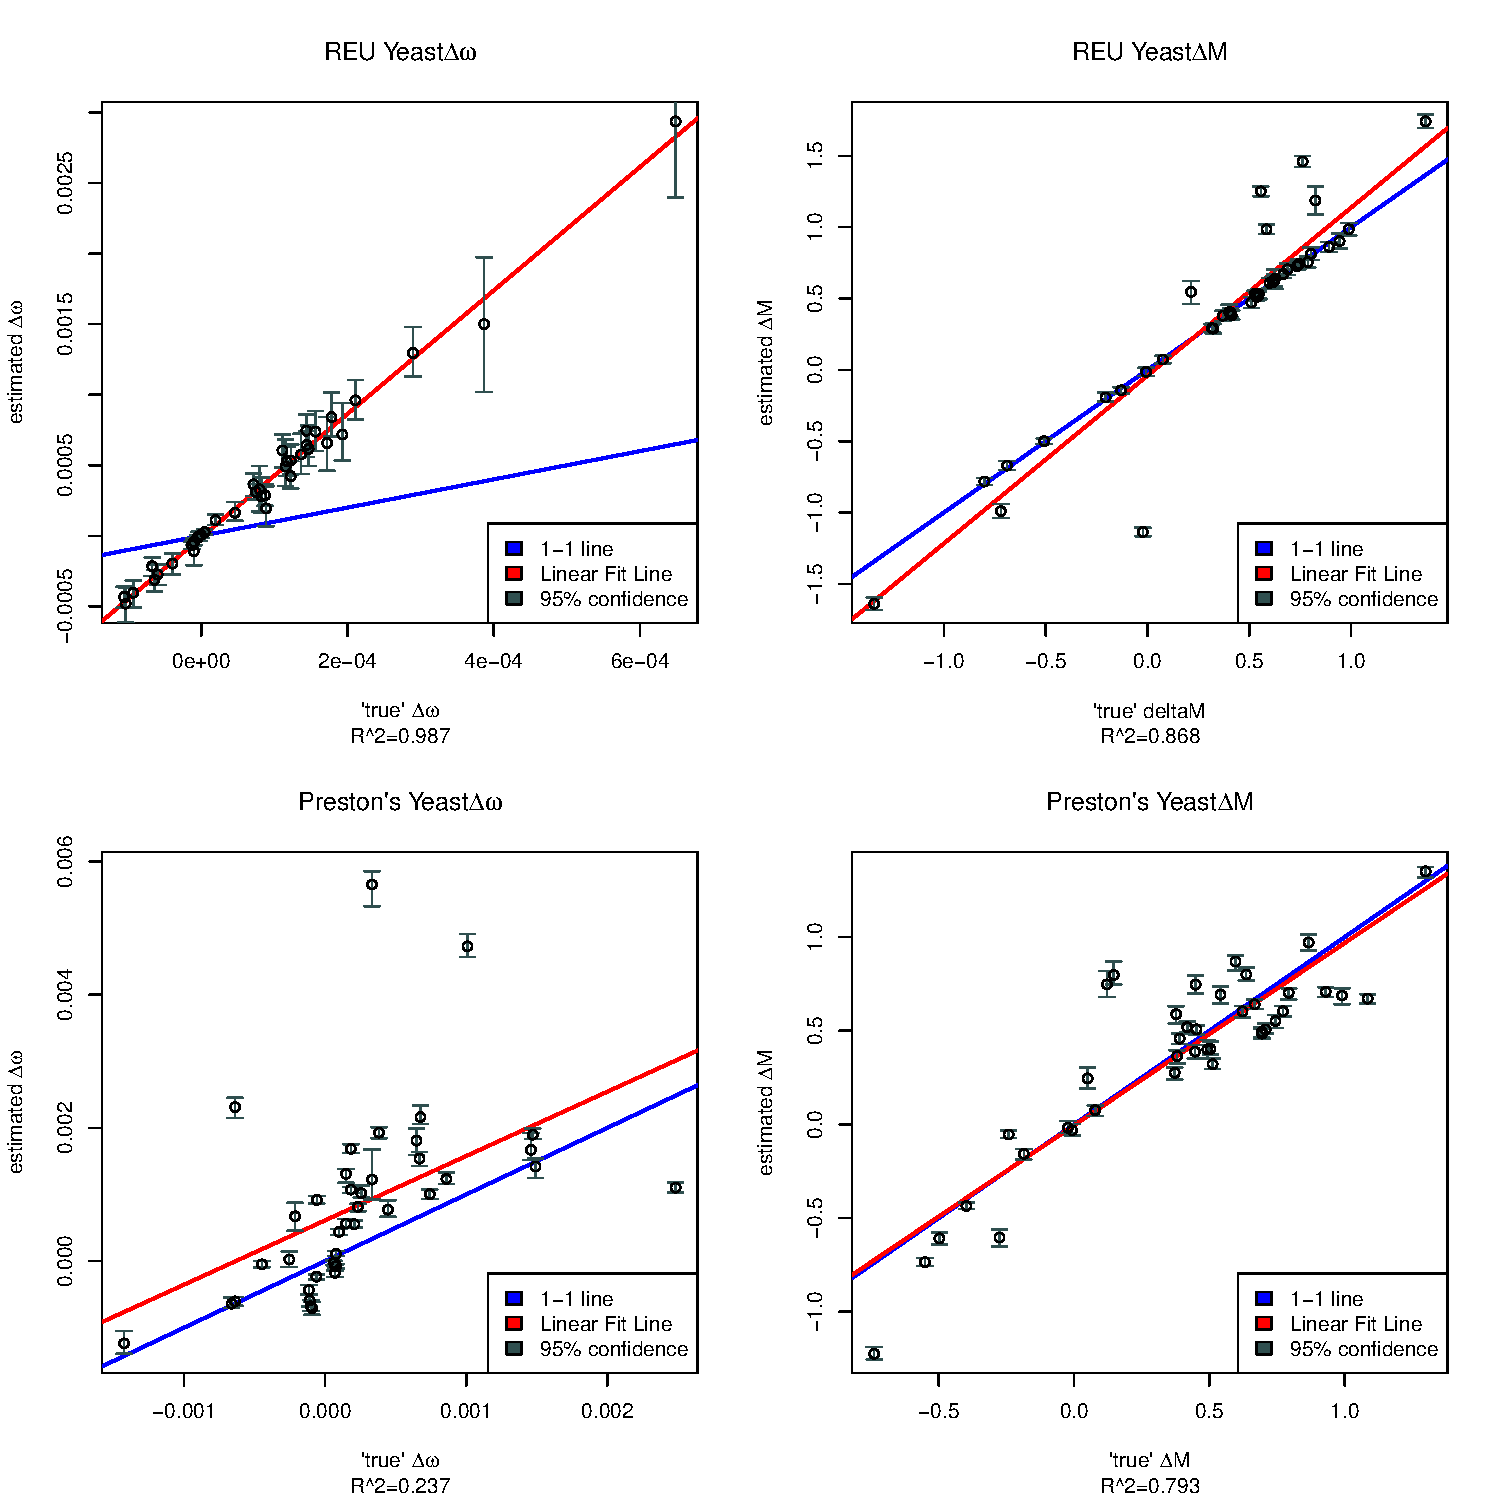
\includepdf[pages={1}]{data/1105_sidebyside.pdf}

\subsubsection{Longer Run?}

A longer run creates some interesting results. I did a run that used 7500 samples instead of 750 (which, since I'm thinning by 10, it's actually 75,000 proposals).

Here's the results (Large run is on the left, small run is on the right)

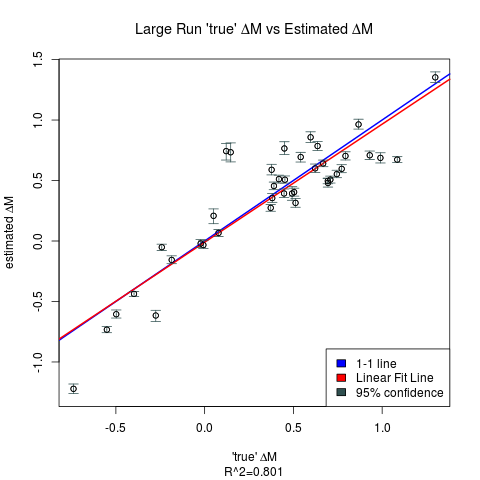
\includegraphics[width=0.5\textwidth]{data/mu_largerun.png}
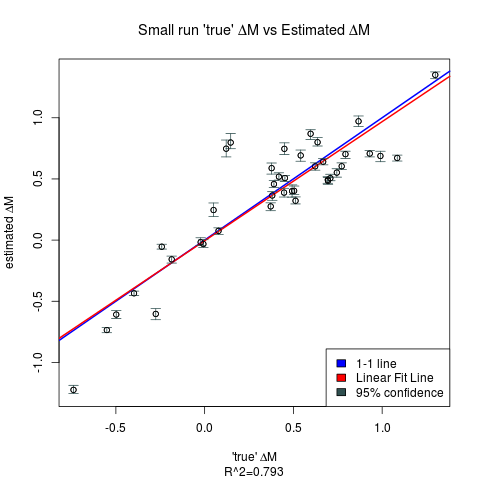
\includegraphics[width=0.5\textwidth]{data/mu_smallrun.png}

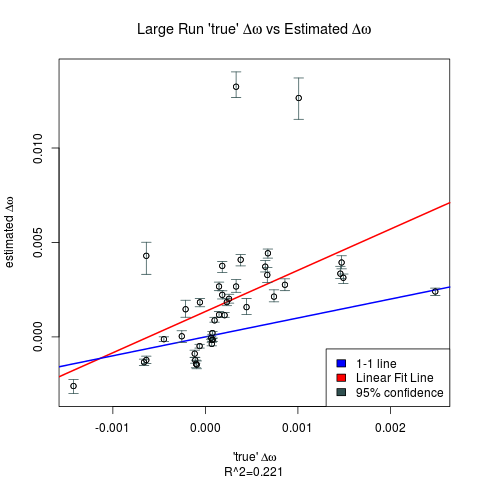
\includegraphics[width=0.5\textwidth]{data/omega_largerun.png}
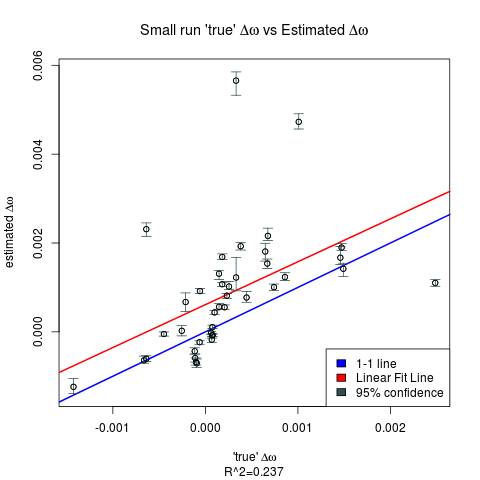
\includegraphics[width=0.5\textwidth]{data/omega_smallrun.png}

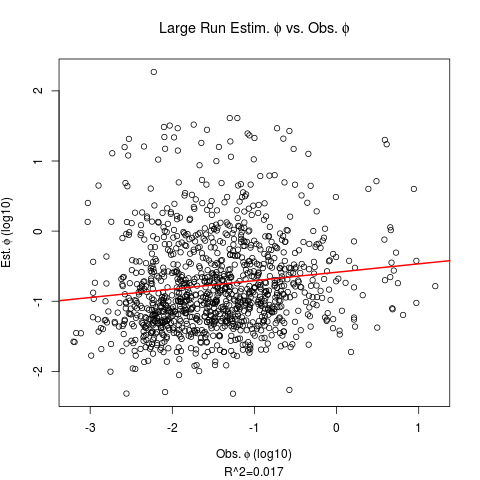
\includegraphics[width=0.5\textwidth]{data/phi_largerun.png}
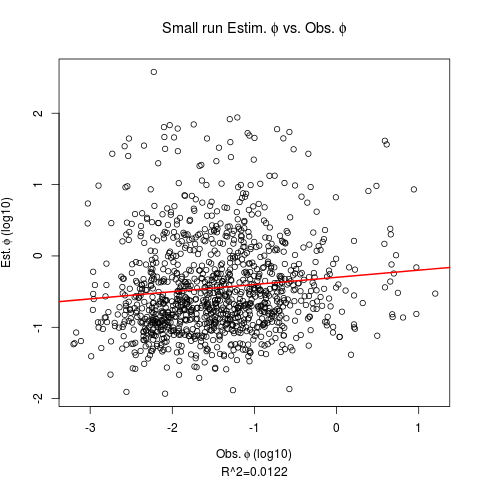
\includegraphics[width=0.5\textwidth]{data/phi_smallrun.png}

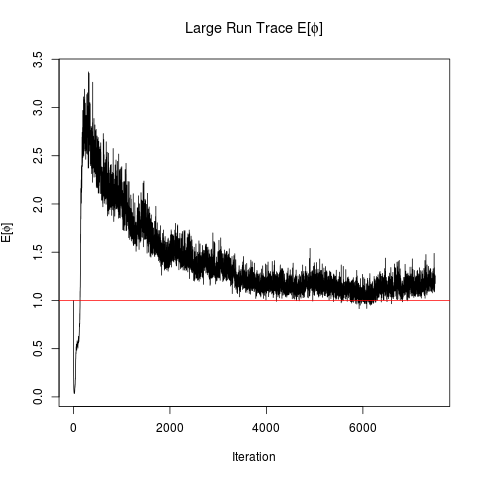
\includegraphics[width=0.5\textwidth]{data/ephi_largerun.png}
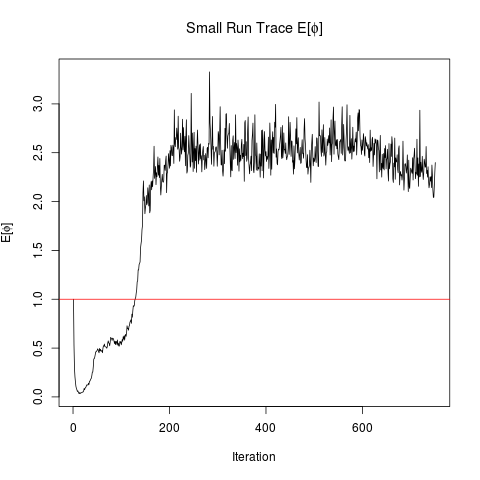
\includegraphics[width=0.5\textwidth]{data/ephi_smallrun.png}

The most relevant thing in my opinion is the E($\phi$) graphs. E($\phi$) should hover around 1. in the small run, it leapt up to 3, and I was concerned this was an inherent problem in the code. But 


\subsection{Visualization}

\subsubsection{'true' values vs simulated values}

Changes have been added to visualize.r, based on other plotting functions.

I've added confidence intervals (the scale of the interval can bet set in visualize.r). Cedric didn't have any functions to do so, but I was able to apply the "plotrix" package. I've also installed that package to "/home/lbrown/cubfits/Dependencies/plotrix". Everyone else should have permissions on that directory, in case someone wants to use my edited visualize.r function.




\subsection{Parallelize the Code}

\subsubsection{getOption(``mc.cores")}
How to set the number of cores for an mclapply call? mclapply's default number of cores is getOption(``mc.cores",2L);

getOption(``(option)", (value)) returns the value previously set to that (option), or otherwise it returns (value). mc.cores is not set by default. So first, set option(``mc.cores"=Number\_of\_Cores). Then mclapply should correctly get the number of cores.

\subsubsection{Timing}

As expected, we get diminshing returns on adding additional processors

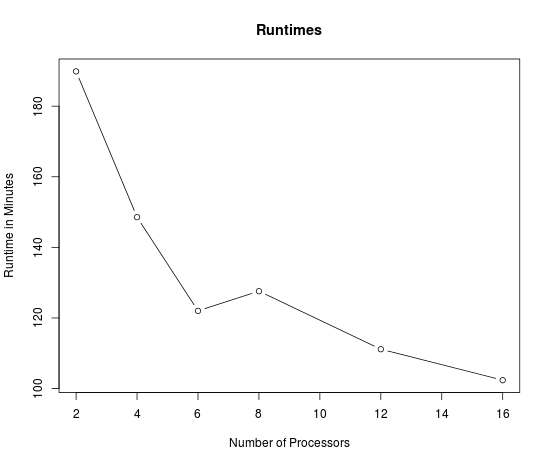
\includegraphics[width=0.5\textwidth]{data/1105runtimes.png}
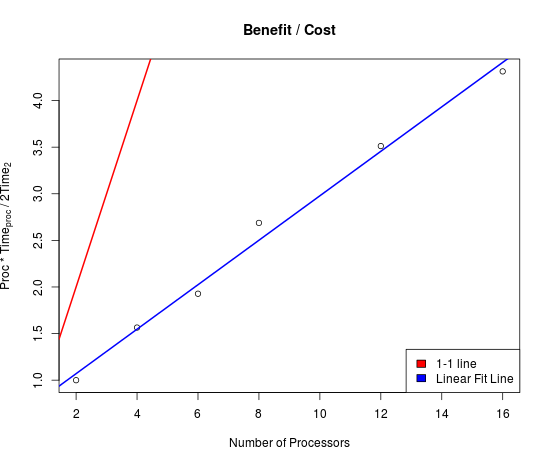
\includegraphics[width=0.5\textwidth]{data/1105timingCostBenefit.png}


\subsection{Add (a1-a2) as a parameter}

In the code, when the posterior probability of a codon is calculated, instead of calculating

\[
\mbox{Pr}(c_i|\phi,i)
=
\frac{
\mbox{exp}[\mbox{M}_i
+ \omega_i(a_1-a_2)y_1
+ \omega_ia_2y_1 i
]
}{
\sum_{u=1}^m
\mbox{exp}[\mbox{M}_i
+ \omega_i(a_1-a_2)y_1
+ \omega_ia_2y_1 i
]
}
\]

Wei Chen calculates

\[
\mbox{Pr}(c_i|\phi,i)
=
\frac{
\mbox{exp}[\mbox{M}_i
%+ \omega_i(a_1-a_2)y_1
- \omega_i\phi i
]
}{
\sum_{u=1}^m
\mbox{exp}[\mbox{M}_i
%+ \omega_i(a_1-a_2)y_1
- \omega_i\phi i
]
}
\]

This was done for a number of reasons. The $y_1$ term is just the aggregate of the effective population, $\phi$, and a scaling term $-q$. Also, the assumption was that $a_1 \approx a_2 = 4$ATP.
To better account for the parameters of the model, we're going to add another parameter called $\Delta a_{12} = (a_1 - a_2)$, and use

\[
\mbox{Pr}(c_i|\phi,i)
=
\frac{
\mbox{exp}[\mbox{ln}
- \omega_i(\Delta a_{12})\phi
- 4\omega_i\phi i
]
}{
\mbox{exp}[\mbox{ln}
\sum_{u=1}^m
\mbox{exp}[\mbox{ln}
- \omega_i(\Delta a_{12})\phi
- 4\omega_i\phi i
]
}
\]

The math part of the change takes place in my.logdmultinomCodOne.r, adding an extra row to xm and multiplying $\omega\phi\Delta a_{12}$, which is baa[2]*tmp.phi*(new parameter)

\subsection{Move to Newton}

Newton uses R 3.0.1, all my dependencies were build under 3.1.1. Newton HAS R 3.1.0, but not 3.1.1.


\subsection{Wrong Names}

It's not just a problem in the chain\$b.Mat data. It's in the my.fitmultinomOne.r

\subsection{Wei Chen's Yeast / Real Yeast Genome}

\subsection{Generate my own simulated yeast, using a reverse engineered cubfits}



\section{Goals for next Month}
\begin{enumerate}
\item Future Goal
\end{enumerate}


\end{document} %End of day document, REMOVE
